\subsection{Alumno}

  \paragraph{}La aplicación permite generar listados de los alumnos a los que
  presta asesoría el usuario \textit{Asesor} que está utilizando la aplicación.
  Una captura de pantalla de este listado se puede ver en la figura
  \ref{capturaPantallaListaAlumnosDeAsesor}.

  \begin{figure}[!ht]
    \begin{center}
      \fbox{
      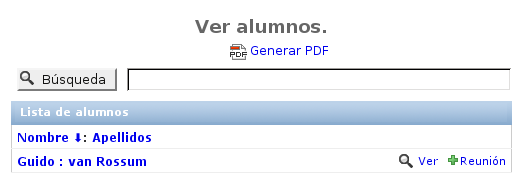
\includegraphics[scale=0.55]{4.Funcionamiento_Aplicacion/4.3.Gestion/4.3.3.Asesor/4.3.3.2.Alumno/lista_alumnos.png}
      }
      \caption{Captura de pantalla de la lista de alumnos a los que asesora el usuario \textit{Asesor}.}
      \label{capturaPantallaListaAlumnosDeAsesor}
    \end{center}
  \end{figure}

  \paragraph{}Desde esta pantalla es posible, además, establecer una reunión
  para un determinado alumno pulsando en el icono \textit{Reunión} que aparece
  al lado de cada alumno de la lista. Este icono se muestra en la figura
  \ref{capturaIconoReunion}.

  \begin{figure}[!ht]
    \begin{center}
      \fbox{
      
\includegraphics[scale=0.6]{4.Funcionamiento_Aplicacion/4.3.Gestion/4.3.3.Asesor/4.3.3.2.Alumno/icono_reunion.png}
      }
      \caption{Captura de pantalla del icono \textit{Reunión}.}
      \label{capturaIconoReunion}
    \end{center}
  \end{figure}
